\documentclass[12pt]{article}
\usepackage[margin=1in]{geometry}
\usepackage[all]{xy}


\usepackage{amsmath,amsthm,amssymb,color,latexsym}
\usepackage{geometry}        
\geometry{letterpaper}    
\usepackage{graphicx}
\usepackage[russian]{babel}
\newtheorem{problem}{Задача}

\newenvironment{solution}[1][\it{Реше\textit{}ние}]{\textbf{#1. } }{$\square$}
\newtheorem{theorem}{Теорема}[section]
\newtheorem{corollary}{Corollary}[theorem]
\newtheorem{lemma}[theorem]{Lemma}
\DeclareMathOperator{\Ima}{Im}
\DeclareMathOperator{\Kera}{Ker}

\begin{document}
\noindent ОВАиТК 2024\hfill Домашнее задание 7 \\
Гаттаров Тимур Б05-304 (25/03/2024)

\hrulefill

\begin{problem}
    Найдите с точностью до изоморфизма все различные абелевы группы порядка 20 (можно представлять группу, как прямое произведение циклических групп).
\end{problem}

\begin{solution}

Воспользумся утверждением, что \textit{любая Абелева группа изоморфна прямому произведению циклических групп. } Вользовавшись Китайской теоремой об остатках, получим что $\mathbb{Z}_{20} \cong \{C_4 \times C_5, C_2 \times C_{10}\} $.


\end{solution}
\begin{problem}
    Существует ли сюръективный гомоморфизм $C_{24} \times C_{18}$ на $C_{16}$?
\end{problem}
\begin{solution}


    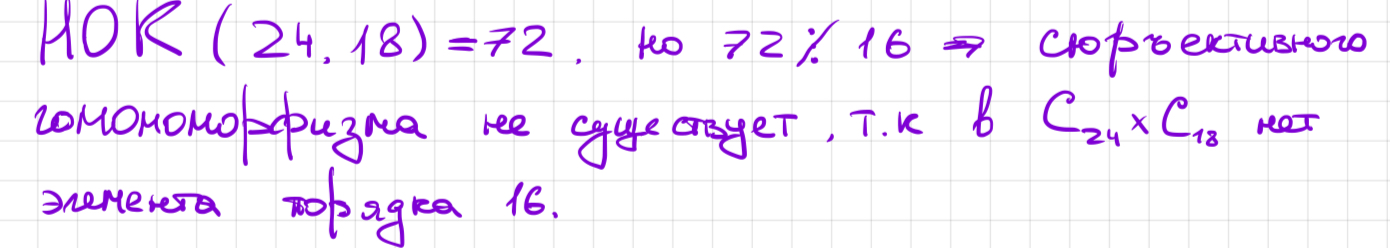
\includegraphics[width = 15cm]{Общая Физика Семинары 2.jpeg}
\end{solution}

\begin{solution}
    Приведём доказательство от противного : пусть гомоморфизм существует. Тогда $\forall a \in C_{24} \times C_{16} \longrightarrow \text{ord} (a) = \text{НОК}(24, 18) = 72$
\end{solution}

\begin{problem}
    Существует ли сюръективный гомоморфизм $C_{16} \times C_{9}$ на $C_{24}$?
\end{problem}

\begin{solution}
    Да, существует, покажем это.
    $$
    \text{НОД}(16, 9) = 144  \text{ }  \vdots \text{ } 24
    $$

    Пусть $c$ - образующий $C_{24}$, тогда
    $$
    (a, e) \longrightarrow c^3, a  \text{ - попрождающий } C_{16}
    $$
    $$
    (e, e) \longrightarrow c^8, a  \text{ - попрождающий } C_{9}
    $$
    Следовательно, этот гомомрфизм будет сюръективаны, так как значения образа покрыты.
\end{solution}

\begin{problem}
    Найдите все элементы группы автоморфизмов $C_{10}$ и укажите, как устроена данная группа (можно показать какой группе она изоморфна).
\end{problem}

\begin{solution}


    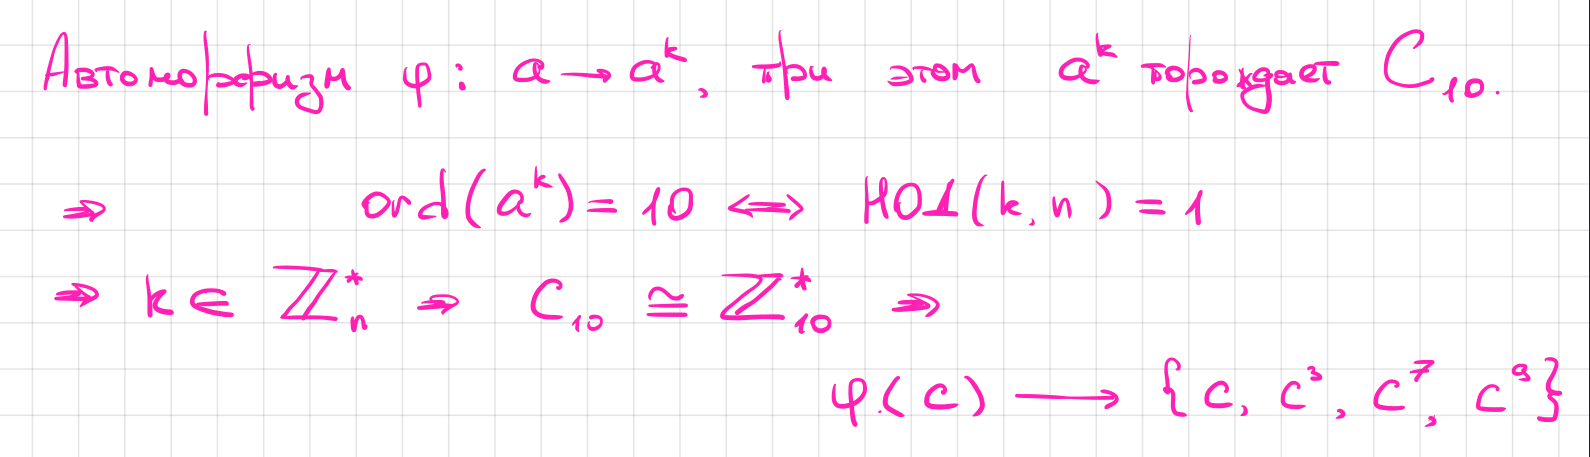
\includegraphics[width = 16cm]{IMG_FAC29663DB78-1.jpeg}
\end{solution}

\begin{problem}
    Найдите все перестановки, коммутирующие с $(123)(4567)$ в $S_{8}$.
\end{problem}

\begin{solution} Нам нужно найти все $\sigma$, такие что  $\sigma \tau = \tau \sigma$ или, что эквивалентно, $\tau = \sigma \tau \sigma^{-1}$. Запишем:
    $$
    \sigma \tau \sigma^{-1} = (\sigma(1) \sigma(2) \sigma(3)) (\sigma(4) \sigma(5) \sigma(6) \sigma(7)) = (123)(4567)
    $$
Заметим, что автоматически $\sigma(8) = 8$. Положим $A := (\sigma(1) \sigma(2) \sigma(3))$ и $B := (\sigma(4) \sigma(5) \sigma(6) \sigma(7))$. Тогда для $A$ возможны случаи:
    \begin{enumerate}
        \item $\sigma(1) = 1, \sigma(2) = 2, \sigma(3) = 3$
        \item $\sigma(1) = 3, \sigma(2) = 1, \sigma(3) = 2$
        \item $\sigma(1) = 2, \sigma(2) = 3, \sigma(3) = 1$
    \end{enumerate}

Аналогично для $B$:

    \begin{enumerate}
        \item $\sigma(4) = 4, \sigma(5) = 5, \sigma(6) = 6, \sigma(7) = 7$
        \item $\sigma(4) = 7, \sigma(5) = 4, \sigma(6) = 5, \sigma(7) = 6$
        \item $\sigma(4) = 6, \sigma(5) = 7, \sigma(6) = 4, \sigma(7) = 5$
        \item $\sigma(4) = 5, \sigma(5) = 6, \sigma(6) = 7, \sigma(7) = 4$
    \end{enumerate}

    Тогда все перестановки, коммутирующие с $(123)(4567)$ в $S_{8}$ есть прямое произведение $A \times B$ в $S_8$. Их всего $\frac{8!}{\frac{8!}{3 \cdot 4}} = 12$
\end{solution}



\end{document}
